\documentclass[12pt]{beamer}
\usepackage{../Estilos/BeamerMAF}
\usepackage{../Estilos/ColoresLatex}
\usetheme{Warsaw}
\usecolortheme{seahorse}
%\useoutertheme{default}
\setbeamercovered{invisible}
% or whatever (possibly just delete it)
\setbeamertemplate{section in toc}[sections numbered]
\setbeamertemplate{subsection in toc}[subsections numbered]
\setbeamertemplate{subsection in toc}{\leavevmode\leftskip=3.2em\rlap{\hskip-2em\inserttocsectionnumber.\inserttocsubsectionnumber}\inserttocsubsection\par}
\setbeamercolor{section in toc}{fg=blue}
\setbeamercolor{subsection in toc}{fg=blue}
\setbeamercolor{frametitle}{fg=blue}
\setbeamertemplate{caption}[numbered]

\setbeamertemplate{footline}
\beamertemplatenavigationsymbolsempty
\setbeamertemplate{headline}{}


\makeatletter
\setbeamercolor{section in foot}{bg=gray!30, fg=black!90!orange}
\setbeamercolor{subsection in foot}{bg=blue!30}
\setbeamercolor{date in foot}{bg=black}
\setbeamertemplate{footline}
{
  \leavevmode%
  \hbox{%
  \begin{beamercolorbox}[wd=.333333\paperwidth,ht=2.25ex,dp=1ex,center]{section in foot}%
    \usebeamerfont{section in foot} \insertsection
  \end{beamercolorbox}%
  \begin{beamercolorbox}[wd=.333333\paperwidth,ht=2.25ex,dp=1ex,center]{subsection in foot}%
    \usebeamerfont{subsection in foot}  \insertsubsection
  \end{beamercolorbox}%
  \begin{beamercolorbox}[wd=.333333\paperwidth,ht=2.25ex,dp=1ex,right]{date in head/foot}%
    \usebeamerfont{date in head/foot} \insertshortdate{} \hspace*{2em}
    \insertframenumber{} / \inserttotalframenumber \hspace*{2ex} 
  \end{beamercolorbox}}%
  \vskip0pt%
}
\makeatother

\makeatletter
\patchcmd{\beamer@sectionintoc}{\vskip1.5em}{\vskip0.8em}{}{}
\makeatother

\newlength{\depthofsumsign}
\setlength{\depthofsumsign}{\depthof{$\sum$}}
\newcommand{\nsum}[1][1.4]{% only for \displaystyle
    \mathop{%
        \raisebox
            {-#1\depthofsumsign+1\depthofsumsign}
            {\scalebox
                {#1}
                {$\displaystyle\sum$}%
            }
    }
}
\def\scaleint#1{\vcenter{\hbox{\scaleto[3ex]{\displaystyle\int}{#1}}}}
\def\scaleoint#1{\vcenter{\hbox{\scaleto[3ex]{\displaystyle\oint}{#1}}}}
\def\bs{\mkern-12mu}


\title{\large{Funciones Gamma y Beta}}
\subtitle{Tema 1 - La física y la geometría}

\author{M. en C. Gustavo Contreras Mayén}
\makeatletter

\setbeamertemplate{footline}
{
  \leavevmode%
  \hbox{%
  \begin{beamercolorbox}[wd=.333333\paperwidth,ht=2.25ex,dp=1ex,center]{section in foot}%
    \usebeamerfont{section in foot} \insertsection
  \end{beamercolorbox}%
  \begin{beamercolorbox}[wd=.333333\paperwidth,ht=2.25ex,dp=1ex,center]{subsection in foot}%
    \usebeamerfont{subsection in foot}  \insertsubsection
  \end{beamercolorbox}%
  \begin{beamercolorbox}[wd=.333333\paperwidth,ht=2.25ex,dp=1ex,right]{date in head/foot}%
    \usebeamerfont{date in head/foot} {T1 - Cuarta presentación} \hspace*{2em}
    \insertframenumber{} / \inserttotalframenumber \hspace*{2ex} 
  \end{beamercolorbox}}%
  \vskip0pt%
}
\makeatother
\date{}

\begin{document}
\maketitle
\fontsize{14}{14}\selectfont
\spanishdecimal{.}

\section*{Contenido}
\frame[allowframebreaks]{\tableofcontents[currentsection, hideallsubsections]}

\section{Integrales como funciones.}
\frame{\tableofcontents[currentsection, hideothersubsections]}
\subsection{Funciones de apoyo}

\begin{frame}
\frametitle{Integrales como funciones}
Las integrales son uno de los medios matemáticos más convenientes con los que se pueden definir nuevas funciones.
\\
\bigskip
\pause
Si el integrando o los límites de integración incluyen parámetros, esos parámetros pueden tratarse como variables y la integral misma como una función de esos parámetros.
\end{frame}
\begin{frame}
\frametitle{Integrales como funciones}
Haremos una revisión de algunas funciones más importantes que normalmente se definen en términos de integrales.
\end{frame}

\subsection*{La función Gamma}

\begin{frame}
\frametitle{De la función Gamma}
La función Gamma $\Gamma (x)$ aparece ocasionalmente en problemas de física tales como:
\pause
\setbeamercolor{item projected}{bg=capri,fg=black}
\setbeamertemplate{enumerate items}{%
\usebeamercolor[bg]{item projected}%
\raisebox{1.5pt}{\colorbox{bg}{\color{fg}\footnotesize\insertenumlabel}}%
}
\begin{enumerate}[<+->]
\item Cálculo de probabilidades en mecánica estadística.
\item La normalización de las funciones de onda para el potencial de Coulomb en mecánica cuántica.
\end{enumerate}
\end{frame}
\begin{frame}
\frametitle{Su uso en la física}
En realidad la función $\Gamma (x)$ tiene pocas aplicaciones directas en física, \pause sin embargo es importante porque nos permite desarrollar otras funciones que si tienen una aplicación directa en la física, como por ejemplo: las funciones de Bessel.
\end{frame}
\begin{frame}
\frametitle{Relación entre las funciones de apoyp}
La relación entre las funciones $\Gamma (x)$ y $B (x, y)$ también nos permitirán expresar de manera más compacta los resultados que se obtendrán al resolver ciertas ecuaciones diferenciales que veremos a lo largo del curso.
\end{frame}
\begin{frame}
\frametitle{Necesidad en el manejo de éstas funciones}
Es por ello que al manejar debidamente estas funciones (y sus variantes), tendremos más herramientas para nuestro objetivo: \pause resolver un problema de la física mediante el uso de funciones especiales, y con ello, interpretar el fenómeno que estudiamos.
\end{frame}
\begin{frame}
\frametitle{Punto importante}
Para el manejo de estas funciones \textocolor{red}{será necesario un trabajo fluido en cuanto a la solución de integrales tanto definidas como indefinidas}, por lo que tendrás oportunidad de ejercitar lo aprendido en los cursos de cálculo.
\end{frame}
\begin{frame}
\frametitle{Punto importante}
Es cierto que existe software matemático (Wolfram, Mathematica, etc.) que te devolverá la solución para algunas integrales, pero confiamos en que utilizarás esas herramientas para corroborar tus resultados, es decir, \pause esperamos que resuelvas \textocolor{darkblue}{a mano} cada una de las integrales que se te presenten.
\end{frame}
\begin{frame}
\frametitle{Punto importante}
Recuerda que es necesario contar con la evidencia de tu trabajo en la solución de un ejercicio, así que como diría un maestro: \enquote{hay que arrastrar el lápiz}.
\end{frame}

% Referencia: Boas (2005) Chap. 11 Special Functions
\subsection{La función factorial.}

\begin{frame}
\frametitle{Definición}
Calculemos el valor de la siguiente integral, para $\alpha > 0$:
\pause
\begin{eqnarray}
\scaleint{6ex}_{\bs 0}^{\infty} e^{-\alpha \, x} \dd{x} = \pause - \dfrac{1}{\alpha} e^{-\alpha \, x}\eval_{0}^{\infty} = \pause \dfrac{1}{\alpha}
\label{eq:ecuacion_02_01_Boas}
\end{eqnarray}
\end{frame}
\begin{frame}
\frametitle{Sobre como escribiremos el argumento}
Con el fin de mantener una buena legibilidad, escribiremos el argumento de la función exponencial como superíndice $e^{-\alpha \, x}$, pero si el argumento es extenso, la función se escribirá como $\exp(-\alpha \, x)$.
\end{frame}
\begin{frame}
\frametitle{Manejando la expresión}
Diferenciamos con respecto a $\alpha$ ambos lados de la ec. (\ref{eq:ecuacion_02_01_Boas}):
\pause
\begin{eqnarray*}
\begin{aligned}
&\scaleint{6ex}_{\bs 0}^{\infty} - x \, e^{-\alpha \, x} \dd{x} = - \dfrac{1}{\alpha^{2}} \pause
\Rightarrow \scaleint{6ex}_{\bs 0}^{\infty} x \, e^{-\alpha \, x} \dd{x} = \dfrac{1}{\alpha^{2}} \\[0.5em] \pause
&\Rightarrow \scaleint{6ex}_{\bs 0}^{\infty} x^{2} \, e^{-\alpha \, x} \dd{x} = \dfrac{2}{\alpha^{3}} \\[0.5em] \pause
&\Rightarrow \scaleint{6ex}_{\bs 0}^{\infty} x^{3} \, e^{-\alpha \, x} \dd{x} = \dfrac{3!}{\alpha^{4}} \\
& \vdots
\end{aligned}
\end{eqnarray*}
\end{frame}
\begin{frame}
\frametitle{Luego de $n$ diferenciaciones}
La expresión general luego de $n$ pasos de diferenciación con respecto a $\alpha$ es:
\pause
\begin{align}
\scaleint{6ex}_{\bs 0}^{\infty} x^{n} \, e^{-\alpha \, x} \dd{x} = \dfrac{n!}{\alpha^{n+1}}
\label{eq:ecuacion_02_02}
\end{align}
\end{frame}
\begin{frame}
\frametitle{Definiendo un valor}
Haciendo que $\alpha = 1$, se obtiene:
\pause
\begin{align}
\scaleint{6ex}_{\bs 0}^{\infty} x^{n} \, e^{-x} \dd{x} = n! \hspace{1cm} n = 1, 2, 3, \ldots
\label{eq:ecuacion_02_03}
\end{align}
\end{frame}
\begin{frame}
\frametitle{Resultado obtenido}
Así tenemos una integral definida cuyo valor es $n!$ para un entero positivo $n$.
\\
\bigskip
\pause
Usando la ec. (\ref{eq:ecuacion_02_03}) le podemos dar un significado al valor de $0!$: si hacemos $n = 0$, ocurre:
\pause
\begin{eqnarray}
0! = \scaleint{6ex}_{\bs 0}^{\infty} e^{-x} \dd{x} = \pause -e^{x}\eval_{0}^{\infty} = \pause 1
\label{eq:ecuacion_02_04}
\end{eqnarray}
\end{frame}

\subsection{Doble factorial.}

\begin{frame}
\frametitle{Definiendo el doble factorial}
En varios problemas de la física, en particular con los \textocolor{darklavender}{polinomios de Legendre}, encontraremos productos de enteros impares positivos y de pares positivos, por conveniencia, definimos el doble factorial:
\pause
\begin{align}
\begin{aligned}
1 \cdot 3 \cdot 5 \cdots (2 \, n+1) &= (2 \, n+1) !! \\
2 \cdot 4 \cdot 6 \cdots (2 \, n) &= (2 \, n) !!
\end{aligned}
\label{eq:ecuacion_10_33b}
\end{align}
\end{frame}
\begin{frame}
\frametitle{Relación con el factorial}
Que están relacionados con la función factorial:
\pause
\begin{align}
\begin{aligned}
(2 \, n)!! &=  2^{n} \: n! \\[1em]
(2 \, n+1)!! &= \dfrac{(2 \, n+1)!}{2^{n} \, n!}
\end{aligned}
\label{eq:ecuacion_10_33c}
\end{align}
\pause
También se define $(-1)!! = 1$, un caso especial que no se obtiene de la ec. (\ref{eq:ecuacion_10_33c})
\end{frame}

\section{Función Gamma}
\frame{\tableofcontents[currentsection, hideothersubsections]}
\subsection{Definición}

\begin{frame}
\frametitle{Factorial para enteros}
En el desarrollo que hemos hecho, $n$ es un número entero no negativo, es natural definir la función factorial para un $n$ no entero mediante la integral de la ec.(\ref{eq:ecuacion_02_03}).
\\
\bigskip
\pause
No hay ninguna objeción en la notación $n!$ para $n$ no entero, pero es habitual reservar la notación factorial para $n$ entero.
\end{frame}
\begin{frame}
\frametitle{Factorial para no enteros}
Para el caso de una función para evaluar el factorial de un $n$ no entero, entonces llamaremos a esa función: la función gamma $(\Gamma (x))$.
\\
\bigskip
\pause
También es una práctica bastante común reemplazar $n$ por la letra $p$ cuando queremos decir que no es necesariamente un número entero.
\end{frame}
\begin{frame}
\frametitle{Definición}
Siguiendo estas convenciones, se define la función Gamma para cualquier $p > 0$:
\pause
\begin{align}\addtolength{\fboxsep}{5pt}\boxed{
\Gamma (p) = \scaleint{6ex}_{\bs 0}^{\infty} x^{p-1} \, e^{-x} \dd{x}, \hspace{1cm} p > 0}
\label{eq:ecuacion_03_01}
\end{align}
\end{frame}
\begin{frame}
\frametitle{Propiedades de $\Gamma (p)$}
\setbeamercolor{item projected}{bg=darkscarlet,fg=white}
\setbeamertemplate{enumerate items}{%
\usebeamercolor[bg]{item projected}%
\raisebox{1.5pt}{\colorbox{bg}{\color{fg}\footnotesize\insertenumlabel}}%
}
\begin{enumerate}[<+->]
\item Para $0 < p < 1$ la integral (\ref{eq:ecuacion_03_01}) se hace impropia, ya que el término $x^{p-1}$ tiende a infinito en el límite inferior.
\item Para $p > 0$ se tiene una integral que converge.
\item Para $p \leq 0$ la integral diverge y no se puede usar para definir $\Gamma (p)$, más adelante veremos cómo definir  $\Gamma (p)$ para $p \leq 0$.
\end{enumerate}
\end{frame}

\subsubsection{Primeras propiedades}

\begin{frame}
\frametitle{Propiedades de $\Gamma (p)$}
De las ecs. (\ref{eq:ecuacion_03_01}) y (\ref{eq:ecuacion_02_03}), se tiene que:
\pause
\begin{align}
\begin{aligned}
\Gamma (n) &= \scaleint{6ex}_{\bs 0}^{\infty} x^{n-1} \, e^{-x} \dd{x} = (n -1)! \\[1em]
\Gamma (n+1) &= \scaleint{6ex}_{\bs 0}^{\infty} x^{n} \, e^{-x} \dd{x} = n!
\end{aligned}
\label{eq:ecuacion_03_02}
\end{align}
\end{frame}
\begin{frame}
\frametitle{Propiedades de $\Gamma (p)$}
Entonces:
\pause
\begin{align*}
\Gamma (1) &= 0! = 1 \\
\Gamma (2) &= 1! = 1 \\
\Gamma (3) &= 2! = 2 \\
\Gamma (4) &= 3! = 6 \\
&\ldots \\
\Gamma (n) &= n-1!
\end{align*}
Donde el factorial de un entero positivo $n$, es el que conocemos del álgebra.
\end{frame}
\begin{frame}
\frametitle{Ampliando la función}
Al reemplazar $p$ por $p+1$ en la ec. (\ref{eq:ecuacion_03_01}) nos deja:
\pause
\begin{align}
\Gamma (p + 1) = \scaleint{6ex}_{\bs 0}^{\infty} x^{p} \, e^{-x} \dd{x} = p!, \hspace{1cm} p > -1
\label{eq:ecuacion_03_03}
\end{align}
En algunos textos se ocupa la notación factorial $p! = \Gamma (p + 1)$, aunque $p$ es un no entero.
\end{frame}

\subsubsection{Relación de recurrencia}

\begin{frame}
\frametitle{Manejando la expresión}
Al integrar por partes la ec. (\ref{eq:ecuacion_03_03}), haciendo:
\pause
\begin{align*}
x^{p} =  u \hspace{2cm} e^{-x} \dd{x} =  \dd{v}
\end{align*}
\end{frame}
\begin{frame}
\frametitle{Resultado obtenido}
Entonces tenemos que:
\pause
\begin{align*}
\dd{u} &= p \, x^{p-1} \dd{x}, \hspace{1cm} v = - e^{-x} \\[1em]
\Gamma (p+1) &= -x^{p} \, e^{-x} \displaystyle \eval_{0}^{\infty} - \displaystyle \scaleint{6ex}_{\bs 0}^{\infty} \left(-e^{-x} \right) \, p \, x^{p-1} \dd{x} = \\[1em]
&= p \displaystyle \scaleint{6ex}_{\bs 0}^{\infty} x^{p-1} \, e^{-x} \dd{x}
\end{align*}
\end{frame}
\begin{frame}
\frametitle{Identificando la expresión}
Donde reconocemos la integral que define a la función Gamma, entonces obtenemos la regla de recurrencia:  
\pause
\begin{align}\addtolength{\fboxsep}{5pt}\boxed{
\Gamma (p + 1) = p \, \Gamma (p)}
\label{eq:ecuacion_03_04}
\end{align}
Que es de utilidad para simplificar expresiones que involucran a la función $\Gamma (p)$.
\end{frame}

\subsubsection{Función Gamma para \texorpdfstring{$p < 0$}{p < 0}}

\begin{frame}
\frametitle{Para ciertos valores de $p$}
Para valores $p < 0$, la función $\Gamma (p)$ no se ha definido hasta el momento.
\\
\bigskip
\pause
Ocuparemos la relación de recursividad ec. (\ref{eq:ecuacion_03_04}) para resolverla.
\end{frame}
\begin{frame}
\frametitle{Ocupando la expresión}
Entonces:
\pause
\begin{align}\addtolength{\fboxsep}{5pt}\boxed{
\Gamma (p) = \dfrac{1}{p} \, \Gamma (p + 1)}
\label{eq:ecuacion_04_01}
\end{align}
que define la función $\Gamma (p)$ para valores $p < 0$
\end{frame}
\begin{frame}
\frametitle{Ejemplos}
Veamos un par de ejemplos:
\pause
\setbeamercolor{item projected}{bg=denim,fg=desertsand}
\setbeamertemplate{enumerate items}{%
\usebeamercolor[bg]{item projected}%
\raisebox{1.5pt}{\colorbox{bg}{\color{fg}\footnotesize\insertenumlabel}}%
}
\begin{enumerate}[<+->]
\item  Se quiere obtener el valor de $\Gamma (-0.3)$, entonces podemos resolverlo de la siguiente manera:
\begin{align*}
\Gamma (-0.3) = - \dfrac{1}{0.3} \, \Gamma (0.7)
\end{align*}
\item  Se quiere obtener el valor de $\Gamma (-0.3)$, entonces podemos resolverlo de la siguiente manera:
\begin{align*}
\Gamma (-1.3) = - \dfrac{1}{(-1.3)(-0.3)} \, \Gamma (0.7)
\end{align*}
\end{enumerate}
\end{frame}
\begin{frame}
\frametitle{Calculando los valores}
Los valores de la función $\Gamma (p)$ se pueden obtener de tablas, pero lo más práctico es ocupar el software matemático (Wolfram, Mathematica) o lenguajes de programación que incluyen librerías científicas, como \texttt{python}.
\end{frame}
\begin{frame}
\frametitle{Comportamiento de $\Gamma (p)$}
De este y el uso sucesivo de la ec. (\ref{eq:ecuacion_04_01}) se deduce que la función $\Gamma (p)$ tiende a infinito no solo en cero sino también en todos los enteros negativos.
\\
\bigskip
\pause
En los intervalos entre los enteros negativos, alterna valores positivos y negativos, negativo de 0 a -1, positivo de -1 a -2, y así sucesivamente, como puede ver en la siguiente figura (\ref{fig:figura_plot_gamma}).
\end{frame}
\begin{frame}
\frametitle{Gráfica de $\Gamma (p)$}
\begin{figure}[H]
   \centering
   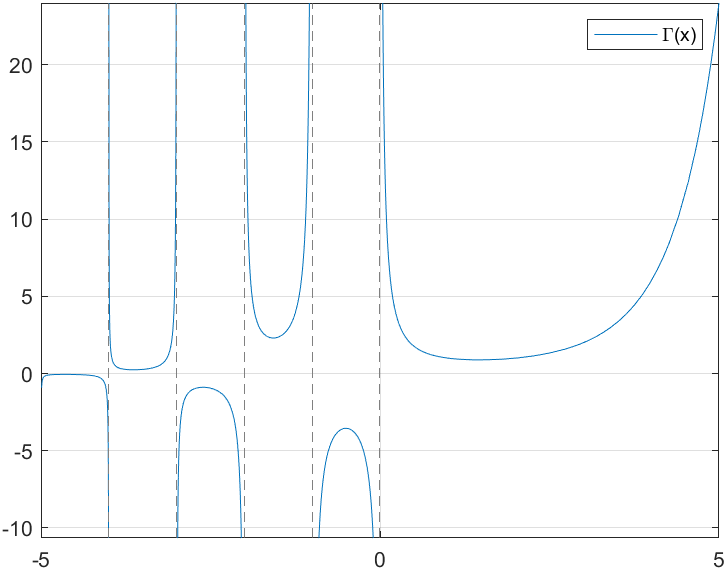
\includegraphics[scale=0.7]{Imagenes/Plot_Gamma.png}
   \caption{Gráfica de la función Gamma $\Gamma (p)$}
   \label{fig:figura_plot_gamma}
\end{figure}
\end{frame}

\subsection{Fórmulas que involucran a \texorpdfstring{$\Gamma (p)$}{G (p)}.}

\begin{frame}
\frametitle{Recuperando más fórmulas}
Como veremos a continuación, el desarrollo de las fórmulas para la función $\Gamma (p)$, se sigue de la definición, por lo que la operación algebraica y de solución de la integral es completamente posible.
\end{frame}
\begin{frame}
\frametitle{Recuperando más fórmulas}
Nos interesa que dispongan de una relación de fórmulas y que puedan ocuparlas en donde sea necesario.
\\
\bigskip
\pause
Aunque las fórmulas son válidas, en el caso que se indique, deberán de demostrar la fórmula que vayan a utilizar.
\end{frame}
\begin{frame}
\frametitle{Evaluando la función}
Evaluemos $\Gamma (1/2)$. Usando la definición:
\pause
\begin{align}
\Gamma \left( \dfrac{1}{2}\right) = \scaleint{6ex}_{\bs 0}^{\infty} \dfrac{1}{\sqrt{t}} \, e^{-t} \dd{t}
\label{eq:ecuacion_05_01}
\end{align}
Toma en cuenta que no importa qué letra usemos para la variable \enquote{muda} de integración en una integral definida.
\end{frame} 
\begin{frame}
\frametitle{Cambiando la variable}
Haciendo el cambio de variable en la ec. (\ref{eq:ecuacion_05_01}):
\pause
\begin{align*}
t = y^{2} \hspace{0.5cm} \Rightarrow \dd{t} = 2 \, y \dd{y}
\end{align*}
\end{frame}
\begin{frame}
\frametitle{Llegamos al resultado}
Entonces tenemos que:
\pause
\begin{align*}
\Gamma \left( \dfrac{1}{2} \right) = \scaleint{6ex}_{\bs 0}^{\infty} \, e^{-y^{2}} \, 2 \, y \dd{y} = 2 \scaleint{6ex}_{\bs 0}^{\infty} \, e^{-y^{2}} \dd{y}
\end{align*}
\end{frame}
\begin{frame}
\frametitle{Usando una variable muda}
Con $x$ como la variable \enquote{muda} de integración:
\pause
\begin{align}
\Gamma \left( \dfrac{1}{2} \right) = 2 \scaleint{6ex}_{\bs 0}^{\infty} \, e^{-x^{2}} \dd{x}
\label{eq:ecuacion_05_02}
\end{align}
\end{frame}
\begin{frame}
\frametitle{Llegando a una integral doble}
Multiplicando las dos integrales de $\Gamma (1/2)$ para luego escribir el resultado como una integral doble:
\pause
\begin{align*}
\left[ \Gamma \left( \dfrac{1}{2} \right) \right]^{2} = 4 \scaleint{6ex}_{\bs 0}^{\infty} \, \scaleint{6ex}_{\bs 0}^{\infty} \, e^{-(x^{2} + y^{2})} \dd{x} \dd{y}
\end{align*}
\end{frame}
\begin{frame}
\frametitle{Resolviendo la integral doble}
Tenemos una doble integral sobre el primer cuadrante de una circunferencia, por lo que es más fácil evaluarla en coordenadas polares:
\pause
\begin{align*}
\left[ \Gamma \left( \dfrac{1}{2} \right) \right]^{2} &= 4 \scaleint{6ex}_{\bs 0}^{\pi/2} \, \scaleint{6ex}_{\bs 0}^{\infty} \, e^{-r^{2}} \, r \dd{r} \dd{\theta} = \\[0.5em]
&= 4 \, \dfrac{\pi}{2} \, \dfrac{e^{-r^{2}}}{-2}\eval_{0}^{\infty} = \\[0.5em]
&= \pi
\end{align*}
\end{frame}
\begin{frame}
\frametitle{Primera expresión}
Entonces obtenemos la primera fórmula:
\pause
\begin{align}\addtolength{\fboxsep}{5pt}\boxed{
\Gamma \left( \dfrac{1}{2} \right) = \sqrt{\pi}}
\label{eq:ecuacion_05_03}
\end{align}
\end{frame}

\subsubsection*{Otras fórmulas}

\begin{frame}
\frametitle{Más expresiones}
A continuación se enlistan algunas de las fórmulas que involucran a la función Gamma, \pause toma en cuenta de que a pesar de que no se demuestra la expresión, en el caso de que la utilices para un ejercicio, deberás de presentar la respectiva demostración.
\end{frame}
\begin{frame}
\frametitle{Expresiones}
{%\fontsize{12}{12}\selectfont
\begin{eqnarray*}
\begin{aligned}
\Gamma (x) &= (x - 1) \, \Gamma(x - 1) \hspace{1cm} x \neq 0, -1, -2, \ldots \\[0.75em] \pause
\Gamma (-x) &= \dfrac{\Gamma (1- x)}{-x} \hspace{1cm} x \neq 0, 1, 2, \ldots \\[0.75em] \pause
\Gamma (x) \, \Gamma (1 - x) &= \dfrac{\pi}{\sin x \, \pi}, \hspace{1.5cm} x \neq 0, \pm 1, \pm 2, \pm 3, \end{aligned}
\end{eqnarray*}
}
\end{frame}
\begin{frame}
\frametitle{Expresiones}
{%\fontsize{12}{12}\selectfont
\begin{eqnarray*}
\begin{aligned}
n! &= \left( \dfrac{n}{e} \right)^{n} \, \sqrt{2 \, \pi \, n} + h \\[0.5em]
&\mbox{con } n = 1, 2, 3, \ldots, \hspace{0.5cm} 0 < \dfrac{h}{n!} < \dfrac{1}{12 \, n} \\[0.5em] \pause
\Gamma \left(n + \dfrac{1}{2} \right) &= \dfrac{1 \cdot 3 \cdot 5 \ldots (2 \, n - 1)\sqrt{\pi}}{2^{n}}, \hspace{0.7cm} n = 1, 2, 3, \ldots
\end{aligned}
\end{eqnarray*}
}
\end{frame}
\begin{frame}
\frametitle{Expresiones}
{%\fontsize{12}{12}\selectfont
\begin{eqnarray*}
\begin{aligned}
\scaleint{6ex}_{\bs 0}^{\infty} t^{a} \, e^{-b \, t^{c}} \dd{t} &= \dfrac{\Gamma \left(\dfrac{a + 1}{c} \right)}{c \, b^{(a+1)/c}}, \\[0.5em]
&\mbox{con } a > -1, \hspace{0.5cm} b > 0, \hspace{0.5cm} c > 0   
\end{aligned}
\end{eqnarray*}
}
\end{frame}

\subsection*{Otras representaciones} \label{seccion:otras_respresentaciones}

\begin{frame}
\frametitle{Diversas representaciones}
Existen al menos tres formas diferentes y convenientes de definir la función Gamma. Se revisarán inicialmente las definiciones así como una serie de consecuencias directas de cada una de ellas.
\end{frame}

\subsubsection{Límite infinito (Euler).}

\begin{frame}
\frametitle{Límite infinito}
La primera definición, llamada de \emph{Euler} es:
\pause
\begin{eqnarray}
\begin{aligned}
\Gamma(z) \equiv \lim_{n \to \infty} &\dfrac{1 \cdot 2 \cdot 3 \cdots n}{z (z + 1) (z + 2) \cdots (z + n)} n^{z}, \\ 
z \neq &0, -1,-2,-3, \ldots
\label{eq:ecuacion_10_01}
\end{aligned}
\end{eqnarray}
\end{frame}
\begin{frame}
\frametitle{Utilidad de la expresión}
Sin pérdida de generalidad, $z$ puede ser real o complejo.
\\
\bigskip
\pause
Esta definición de $\Gamma(z)$ es útil para el desarrollo del producto infinito de Weierstrass de $\Gamma (z)$.
\end{frame}
\begin{frame}
\frametitle{Cambiando la variable}
Reemplazando $z$ con $z + 1$, tenemos:
\pause
\begin{align}
\begin{aligned}[b]
&\Gamma (z + 1) = \\[0.5em]
&= \lim_{n \to \infty} \dfrac{1 \cdot 2 \cdot 3 \cdots n}{(z {+} 1)(z {+} 2)(z {+} 3) \cdots (z {+} n {+} 1)} n^{z {+} 1} = \\[0.5em]
&= \lim_{n \to \infty} \dfrac{n \, z}{z {+} n {+} 1} \: \dfrac{1 \cdot 2 \cdot 3 \cdots n}{z (z {+} 1)(z {+} 2)(z {+} 3) \cdots (z {+} n)} n^{z} \\[0.5em]
&= z \: \Gamma (z)
\label{eq:ecuacion_10_02}
\end{aligned}
\end{align}
\fontsize{12}{12}\selectfont
Esta es la relación funcional básica para la función Gamma.
\end{frame}
\begin{frame}
\frametitle{Característica de la expresión}
Debe notarse que es una ecuación de diferencias. Se ha demostrado que la función Gamma es una de una clase general de funciones que no satisfacen ninguna ecuación diferencial con coeficientes racionales.
\end{frame}
\begin{frame}
\frametitle{De la relación con otra función especial}
Específicamente, la función Gamma es una de las pocas funciones de la física matemática que no satisface tanto la ecuación diferencial hipergeométrica como la ecuación hipergeométrica confluente (que estudiaremos en el \emph{Tema 5 - Funciones Especiales}).
\end{frame}
\begin{frame}
\frametitle{Revisando la expresión}
De la definición:
\pause
\begin{align}
\Gamma (1) = \lim_{n \to \infty} \dfrac{1 \cdot 2 \cdot 3 \cdots n}{1 \cdot 2 \cdot 3 \cdots n \, (n + 1)} \: n = 1
\label{eq:ecuacion_10_03}
\end{align}
\end{frame}
\begin{frame}
\frametitle{Ocupando otra expresión}
Usando de la ecuación (\ref{eq:ecuacion_10_02}), tenemos:
\pause
\begin{align}
\begin{aligned}
\Gamma (2) &= 1 \\
\Gamma (3) &=  2 \: \Gamma(2) =  2 \\
\vdots \\
\Gamma (n) &= 1 \cdot 2 \cdot 3 \cdots (n-1) =  (n-1)!
\label{eq:ecuacion_10_04}
\end{aligned}
\end{align}
\end{frame}

\subsection{Integral definida (Euler)}

\begin{frame}
\frametitle{Segunda definición}
Una segunda definición es la llamada forma de Euler:
\pause
\begin{align}
\Gamma (z) \equiv \scaleint{6ex}_{\bs 0}^{\infty} e^{-t} \: t^{z - 1} \, \dd t, \hspace{1.5cm} \Re(z) > 0
\label{eq:ecuacion_10_05}
\end{align}
La restricción en $z$ es necesaria para prevenir la divergencia de la integral.
\end{frame}
\begin{frame}
\frametitle{Variantes de $\Gamma (z)$}
Cuando la función Gamma aparece en problemas de la física, a menudo tiene una variante:
\pause
\begin{align}
\Gamma (z) &= 2 \: \scaleint{6ex}_{\bs 0}^{\infty} \exp(-t^{2}) \: t^{2 \, z - 1} \dd{t}, \hspace{1cm} \Re(z) > 0  \label{eq:ecuacion_10_06} \\
\Gamma (z) &=  \scaleint{6ex}_{\bs 0}^{1} \left[ \ln\left(\dfrac{1}{t} \right) \right]^{z - 1} \dd{t}, \hspace{1cm} \Re (z) > 0 \label{eq:ecuacion_10_07}
\end{align}
\end{frame}
\begin{frame}
\frametitle{Recuperando otra función}
Cuando $z = 1/2$, la ecuación (\ref{eq:ecuacion_10_06}) es la función de error gaussiana, que nos devuelve el siguiente resultado interesante:
\pause
\begin{align}
\Gamma (1/2) = \sqrt{\pi}
\label{eq:ecuacion_10_08}
\end{align}
\end{frame}
\begin{frame}
\frametitle{Demostrando la relación}
Para mostrar la equivalencia de esas dos definiciones, las ecuaciones (\ref{eq:ecuacion_10_01}) y (\ref{eq:ecuacion_10_05}) consideremos la función de dos variables:
\pause
\begin{align}
F(z, n) = \scaleint{6ex}_{\bs 0}^{n} \left( 1 - \dfrac{t}{n} \right)^{n} \: t^{z - 1} \dd{t}, \hspace{1.5cm} \Re(z) > 0
\label{eq:ecuacion_10_09}
\end{align}
con $n$ entero positivo.
\end{frame}
\begin{frame}
\frametitle{Revisando la expresión}
Ya que:
\pause
\begin{align}
\lim_{n \to \infty} \left( 1 - \dfrac{t}{n} \right)^{n} \equiv e^{-t}
\label{eq:ecuacion_10_10}
\end{align}
\end{frame}
\begin{frame}
\frametitle{Ocupando al definición}
De la definición de función exponencial:
\pause
\begin{equation}
\begin{aligned}[b]
&\lim_{n \to \infty} F(z, n) = F (z, \infty) = \\[0.5em]
&= \scaleint{6ex}_{\bs 0}^{\infty} \exp(-t) \: t^{z - 1} \dd{t} \equiv \Gamma (z)
\end{aligned}
\label{eq:ecuacion_10_11}
\end{equation}
por la ecuación (\ref{eq:ecuacion_10_05}).
\end{frame}
\begin{frame}
\frametitle{Regresando a la expresión}
Regresando a $F (z, n)$, evaluamos sucesivamente la integral por partes, hacemos de manera conveniente $u = t/n$. Entonces:
\pause
\begin{align}
F (z, n) = n^{2} \: \scaleint{6ex}_{\bs 0}^{1} (1-u)^{n} \: u^{z-1} \dd{u}
\label{eq:ecuacion_10_12}
\end{align}
\end{frame}
\begin{frame}
\frametitle{Integrando la expresión}
Integrando por partes:
\pause
\begin{eqnarray}
\begin{aligned}[b]
&\dfrac{F (z, n)}{n^{2}} =  (1-u)^{n} \: \dfrac{u^{z}}{z} \eval_{0}^{1} + \\
&+ \dfrac{n}{z} \: \scaleint{6ex}_{\bs 0}^{1} (1-u)^{n-1} \: u^{z} \dd{u}
\end{aligned}
\label{eq:ecuacion_10_13}
\end{eqnarray}
\end{frame}
\begin{frame}
\frametitle{Repitiendo el cálculo}
Repitiendo esto cada vez con el integrando se anula en ambos extremos, por lo que:
\pause
\begin{align}
\begin{aligned}[b]
F (z, n) &= n^{z} \: \dfrac{n(n-1) \cdots 1}{z \, (z+1) \cdots (z+n-1)} \scaleint{6ex}_{\bs 0}^{1} u^{z+n-1} \dd{u} \\[0.5em]
&= \dfrac{1 \cdot 2 \cdot 3 \cdots n}{z \, (z+1)(z+2) \cdots (z+n)} \: n^{z}
\label{eq:ecuacion_10_14}
\end{aligned}
\end{align}
\end{frame}
\begin{frame}
\frametitle{Identificando el resultado}
Que es idéntico con la expresión del lado derecho de la ecuación (\ref{eq:ecuacion_10_01}). De aquí que:
\pause
\begin{equation}
\lim_{n \to \infty} F(z, n) = F(z, \infty) \equiv \Gamma (z)
\label{eq:ecuacion_10_15}
\end{equation}
\end{frame}

\subsection{Producto infinito (Weierstrass)}

\begin{frame}
\frametitle{Tercera definición}
La tercera forma conocida como forma de Weierstrass es:
\pause
\begin{align}
\dfrac{1}{\Gamma (z)} \equiv z \:  e^{\gamma \, z} \: \prod_{n=1}^{\infty} \left( 1 + \dfrac{z}{n} \right) \: e^{-z/n}
\label{eq:ecuacion_10_16}
\end{align}
donde $\gamma$ es la constante de \emph{Euler-Mascheroni}:
\begin{align}
\gamma = 0.5772156619
\label{eq:ecuacion_10_17}
\end{align}
\end{frame}
\begin{frame}
\frametitle{Resultado de utilidad}
De esta definición de producto infinito de $\Gamma (z)$, se obtiene una identidad importante:
\pause
\begin{align}
\Gamma (z) \: \Gamma (1 - z) = \dfrac{\pi}{\sin z \, \pi}
\label{eq:ecuacion_10_23}
\end{align}
\end{frame}
\begin{frame}
\frametitle{Otro resultado}
Así también la \textbf{fórmula de duplicación de Legendre}:
\pause
\begin{align}
\Gamma (1 + z) \: \Gamma (z + \frac{1}{2}) = 2^{-2 \, z} \: \sqrt{\pi} \: \Gamma (2 \, z + 1)
\label{eq:ecuacion_10_24b}
\end{align}
\end{frame}
\begin{frame}
\frametitle{Polos en la función}
La definición de Weierstrass muestra directamente que $\Gamma (z)$ tiene polos simples en $z = 0, -1, -2, -3, \ldots$ y que $[\Gamma (z)]^{-1}$ no tiene polos en el plano complejo finito, lo que significa que $\Gamma (z)$ no tiene ceros.
\end{frame}

\subsection{Funciones Digamma y Poligamma}

\subsection*{La función Digamma}

\begin{frame}
\frametitle{Función Digamma}
No es conveniente manejar las derivadas de las funciones Gamma o factorial de manera directa, como se definieron en la sección (\ref{seccion:otras_respresentaciones}).
\end{frame}
\begin{frame}
\frametitle{Ajuste en la expresión}
Para evitar ese manejo, lo que se hace es tomar el logaritmo natural de la función factorial (\ref{eq:ecuacion_10_01}), cambiando el producto a una suma y luego se realiza la diferenciación, es decir:
\pause
\begin{align}
z! = \lim_{n \to \infty} \dfrac{n!}{(z + 1)(z + 2) \ldots (z + n)} \, n^{z}
\label{eq:ecuacion_10_36}
\end{align}
\end{frame}
\begin{frame}
\frametitle{Tomando el logaritmo natural}
Que al tomar el logaritmo natural, resulta:
\pause
\begin{align}
\begin{aligned}
\ln (z!) &= \lim_{n \to \infty} \big[ \ln (n!) + z \, \ln n - \ln (z + 1) + \\[0.5em]
&- \ln (z + 2) - \ldots - \ln (z + n) \big]
\end{aligned}
\label{eq:ecuacion_10_37}
\end{align}
en donde el logaritmo del límite es igual al límite del logaritmo
\end{frame}
\begin{frame}
\frametitle{Diferenciando la expresión}
Al diferenciar con respecto a $z$, se obtiene:
\pause
\begin{align}
\begin{aligned}[b]
&\dv{\ln (z!)}{z} \equiv \psi(z + 1) = \\[0.5em]
&=\lim_{n \to \infty} \bigg[ \ln n {+} z - \dfrac{1}{(z {+} 1)} - \dfrac{1}{(z {+} 2)} \ldots - \dfrac{1}{(z {+} n)} \bigg]
\end{aligned}
\label{eq:ecuacion_10_38}
\end{align}
\end{frame}
\begin{frame}
\frametitle{La función digamma}
La cual define a la \emph{función digamma}. De la expresión para la constante de Euler-Mascheroni, la ec. (\ref{eq:ecuacion_10_38}) se puede reescribir como:
\pause
\begin{align}
\begin{aligned}[b]
\psi (z + 1) &= - \gamma - \sum_{n=1}^{\infty} \left( \dfrac{1}{z + n} - \dfrac{1}{n} \right) = \\[0.5em]
&= -\gamma + \sum_{n=1}^{\infty} \dfrac{z}{n (n + z)}
\end{aligned}
\label{eq:ecuacion_10_39}
\end{align}
\end{frame}

\subsection*{Función Poligamma.}

\begin{frame}
\frametitle{Diferenciando nuevamente}
La función Digamma se puede diferenciar de manera iterativa, dando origen a la función Poligamma:
\pause
\begin{align}
\begin{aligned}
&\ntilde{\psi}{m} (z + 1) \equiv \dv[m+1]{z} \ln(z!) = \\[0.5em]
&= (-1)^{m+1} \, m! \,\sum_{n=1}^{\infty} \dfrac{1}{(z + n)^{m+1}}, \hspace{1cm} m = 1, 2, 3, \ldots
\end{aligned}
\label{eq:ecuacion_10_41}
\end{align}
\end{frame}
\section{Función Beta}
\frame[allowframebreaks]{\tableofcontents[currentsection, hideothersubsections]}
\subsection{Definición}
\begin{frame}[fragile]
\frametitle{Definición de la función Beta}
La función Beta se define por la siguiente integral:
\begin{align} \addtolength{\fboxsep}{5pt}\boxed{
\begin{gathered}
B(p, q) = \scaleint{6ex}_{\bs 0}^{1} x^{p-1} \, (1- x )^{q-1} \dd{x}, \\
\mbox{con }  p > 0, q > 0
\end{gathered}
}
\label{eq:ecuacion_06_01}
\end{align}
\pause
Existen una serie de fórmulas para la función Beta que es conveniente conocer, todas ellas derivadas de la definición.
\end{frame}
\begin{frame}
\frametitle{Fórmulas para $B(p, q)$}
Si cambiamos el rango de integración de la ec. (\ref{eq:ecuacion_06_01}), haciendo $x = y/a$, entonces $x = 1$ corresponde a $y = a$, por lo que tenemos:
\begin{align} \addtolength{\fboxsep}{5pt}\boxed{
\begin{aligned}
B (p, q) &= \scaleint{6ex}_{\bs 0}^{a} \left( \dfrac{y}{a}\right)^{p-1} \, \left( 1 - \dfrac{y}{a}\right)^{q-1} \dfrac{\dd{y}}{a} \\[0.5em]
&= \dfrac{1}{a^{p+q-1}} \scaleint{6ex}_{\bs 0}^{a} y^{p-1} \, (a - y)^{q-1} \dd{y}
\end{aligned}
\label{eq:ecuacion_06_03}
}
\end{align}
\end{frame}
\subsection{Fórmula trigonométrica de \texorpdfstring{$B(p,q)$}{B(p, q)}}
\begin{frame}
\frametitle{Fórmula trigonométrica de $B(p,q)$}
Para obtener la forma trigonométrica de la función Beta, hacemos el cambio de variable $x = \sin^{2} \theta$, así
\begin{align*}
\dd{x} &= 2 \, \sin \theta \, \cos \theta \dd{\theta} \\[1em]
(1 - x) &= 1 - \sin^{2} \theta = \cos^{2} \theta \\[1em]
x &= 1 \hspace{0.3cm} \Rightarrow \hspace{0.3cm} \theta = \pi/2
\end{align*}
\end{frame}
\begin{frame}
\frametitle{Fórmula trigonométrica de $B(p, q)$}
Haciendo las sustituciones en la ec. (\ref{eq:ecuacion_06_01}):
{\fontsize{12}{12}\selectfont
\begin{align}
B(p, q) = \scaleint{6ex}_{\bs 0}^{\pi/2} \left( \sin^{2} \theta \right)^{p-1} \, \left( \cos^{2} \theta \right)^{q-1} \, 2 \, \sin \theta \, \cos \theta \dd{\theta}
\end{align}}
\pause
Simplificando la expresión llegamos a:
{\fontsize{12}{12}\selectfont
\begin{align}
\addtolength{\fboxsep}{5pt}\boxed{B(p, q) = 2 \, \scaleint{6ex}_{\bs 0}^{\pi/2} \left( \sin^{2} \theta \right)^{2p-1} \, \left( \cos^{2} \theta \right)^{2q-1} \dd{\theta}}
\label{eq:ecuacion_06_04}
\end{align}}
\end{frame}
\begin{frame}
\frametitle{Otra fórmula para $B(p, q)$}
Con el cambio de variable en la ec. (\ref{eq:ecuacion_06_01})
\begin{align*}
x = \dfrac{y}{(1 + y)}
\end{align*}
\pause
Se puede demostrar que
\begin{align}
\addtolength{\fboxsep}{5pt}\boxed{B(p, q) = \scaleint{6ex}_{\bs 0}^{\infty} \dfrac{y^{p-1}}{(1 + y)^{p+q}} \dd{y}}
\label{eq:ecuacion_06_05}
\end{align}   
\end{frame}
\begin{frame}
\frametitle{Otras fórmulas}
Como en el caso de la función $\Gamma (x)$, las fórmulas que se presentan para $B(p, q)$ se demuestran a partir de la definición y de un manejo algebraico, por lo que en caso de que utilices alguna en la solución de un ejercicio, tendrás que demostrar la fórmula.
\end{frame}
\begin{frame}
\frametitle{Otras fórmulas}
\begin{align*}
B (x, y) &= B (y, x) \\[1em]
B (x, 2-x) &= \dfrac{\pi}{\sin x \, \pi}, \hspace{1.5cm} 0 < x < 1   
\end{align*}
\end{frame}
\subsection{La funión Beta en términos de Gamma}
\begin{frame}
\frametitle{La función $B(p, q)$ en términos de $\Gamma (p)$}
La función Beta se expresa en términos de la función Gamma de la siguiente manera:
\begin{align}
\addtolength{\fboxsep}{5pt}\boxed{B(p, q) = \dfrac{\Gamma(p) \, \Gamma(q)}{\Gamma (p + q)}}
\label{eq:ecuacion_07_01}
\end{align}
Esta fórmula nos ayuda a evaluar una función $B (p, q)$ en términos de funciones $\Gamma$. \textbf{Nota: } también es fácil demostrar la expresión, para que en el caso de que la utilices, realices el ejercicio.
\end{frame}
\section{Ejemplos}
\frame[allowframebreaks]{\tableofcontents[currentsection, hideothersubsections]}
%Referencia: Farrell - Solved Problems in Analysis as Applied to Gamma Function II-39
\subsection{Longitud de una lemniscata}
\begin{frame}
\frametitle{Longitud de una leminiscata}
Usando la función Gamma, calcula la longitud de la lemniscata
\begin{align*}
\rho^{2} = a^{2} \, \cos 2 \theta
\end{align*}
\end{frame}
\begin{frame}
\frametitle{Longitud de una leminiscata}
\begin{wrapfigure}{r}{0.55\textwidth}
    \centering
    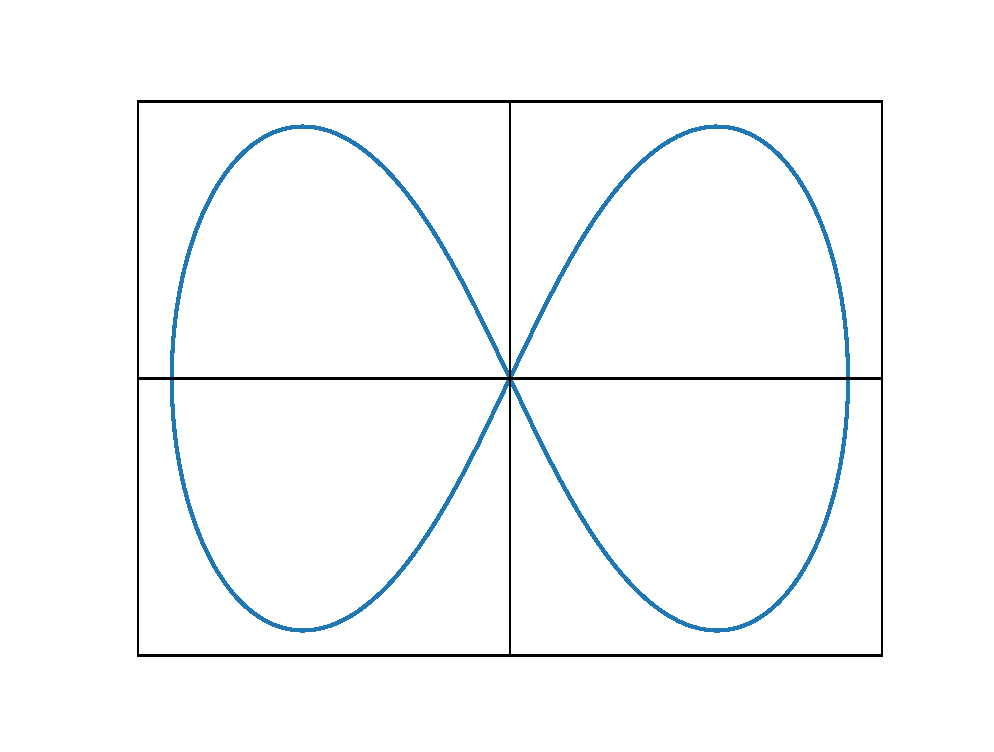
\includegraphics[scale=0.35]{Imagenes/plot_leminscata_01.eps}
    \caption{Gráfica de la lemniscata.}
    \label{fig:figura_lemniscata}
\end{wrapfigure}
La curva se parece a un ocho invertido, teniendo al eje x como eje de simetría, pasa en dos ocasiones por el origen, como se puede ver en la figura (\ref{fig:figura_lemniscata})
\end{frame}
\begin{frame}
\frametitle{Tomando la simetría del problema}
Para esta curva, por simetría se tiene la misma longitud en cada uno de los cuatro cuadrantes, por lo que podemos calcular la longitud en el primer cuadrante y luego multiplicarla por cuatro.
\end{frame}
\begin{frame}
\frametitle{Tomando la simetría del problema}
Los puntos donde la curva cruza el eje $x$ en el origen son aquellos para los cuales el argumento del coseno es un múltiplo entero, impar de $\pi / 2$. 
\\
\bigskip
Para el tramo en el primer cuadrante, tomamos $0 \leq \theta \leq \pi/4$.
\end{frame}
\begin{frame}
\frametitle{Resolviendo el problema}
La longitud de la curva en coordenadas polares es
\begin{align*}
s = \scaleint{6ex}_{\bs \alpha}^{\beta} \left[ \rho^{2} + \left( \dv{\rho}{\theta} \right)^{2} \right]^{1/2} \dd{\theta}
\end{align*}
\pause
Como $\rho^{2} = a^{2} \, \cos 2 \theta$, tenemos que:
\begin{align*}
\left( \dv{\rho}{\theta} \right)^{2} = \dfrac{a^{4} \, \sin^{2} 2 \theta}{a^{2} \, \cos 2 \theta}
\end{align*}
\end{frame}
\begin{frame}
\frametitle{Resolviendo el problema}
Entonces:
\begin{align*}
\dfrac{1}{4} \, s &= \scaleint{6ex}_{\bs {0}}^{\pi/4} \left( a^{2} \, \cos 2 \theta + \dfrac{a^{4} \, \sin^{2} 2 \theta}{\cos 2 \theta} \right)^{1/2} \dd{\theta} = \\[1em]
&= \scaleint{6ex}_{\bs {0}}^{\pi/4} a \, \cos^{-1/2} 2 \theta \dd{\theta}
\end{align*}
\end{frame}
\begin{frame}
\frametitle{Resolviendo al integral}
Haciendo un cambio de variable, es posible llevar esta integral a uno forma de la función Beta con integral.
\\
\bigskip
Sea $2 \theta = t$. Por lo que el intervalo de integración ahora va de $0$ a $\pi/2$.
\end{frame}
\begin{frame}
\frametitle{Resolviendo la integral}
Por tanto:
\begin{align*}
\scaleint{6ex}_{\bs 0}^{\pi/4} a \, \cos^{-1/2} \, 2 \, \theta \dd{\theta} = \dfrac{a}{2} \scaleint{6ex}_{\bs {0}}^{\pi/2} \cos^{-1/2} \, t \, \sin^{0} t \dd{t}
\end{align*}
\end{frame}
\begin{frame}
\frametitle{Resolviendo la integral}
De uno de los resultados para la función Beta:
\begin{align*}
B(x, y) = \scaleint{6ex}_{\bs {0}}^{\pi/2} 2 \, \sin^{2x-1} \theta \, \cos^{2y-1} \theta \dd{\theta}
\end{align*}
\pause
por tanto
\begin{align*}
\dfrac{1}{4} \, s &= \scaleint{6ex}_{\bs {0}}^{\pi/4} a \, \cos^{-1/2} 2 \theta \dd{\theta} =  \\[0.5em]
&= \dfrac{a}{2} \scaleint{6ex}_{\bs {0}}^{\pi/2} \cos^{-1/2} t \, \sin^{0} t \dd{t}
\end{align*}
\end{frame}
\begin{frame}
\frametitle{Resolviendo la integral}
Encontramos entonces que
\begin{align*}
\dfrac{1}{4} \, s &= \dfrac{a}{2} \, \dfrac{1}{2} \, B \, \left(\dfrac{1}{4}, \dfrac{1}{2} \right) = \\[1em]
&= \dfrac{a}{4} B\left(\dfrac{1}{4}, \dfrac{1}{2} \right)
\end{align*}
\pause
\fontsize{12}{12}\selectfont
La longitud completa de la lemniscata se obtiene al multiplicar el resultado anterior por cuatro, además ocupamos la fórmula que relaciona la función Beta con la función Gamma.
\end{frame}
\begin{frame}
\frametitle{Solución al problema}
Así tenemos el resultado:
\begin{eqnarray*}
s &=& a \, B\left(\dfrac{1}{4}, \dfrac{1}{2} \right) = \dfrac{a \, \Gamma \left( \dfrac{1}{4} \right) \, \Gamma \left( \dfrac{1}{2} \right) }{\Gamma \left( \dfrac{3}{4} \right)} = \\ \pause
&=& \dfrac{4 \, a \, \Gamma \left( \dfrac{5}{4} \right) \sqrt{\pi}}{\dfrac{4}{3} \, \Gamma \left( \dfrac{7}{4} \right)} \pause \cong 5.2 \, a
\end{eqnarray*}
\end{frame}
\subsection{Período de oscilación de un péndulo.}
\begin{frame}
\frametitle{Problema de mecánica}
Se nos pide calcular el período de oscilación de un péndulo simple que oscila en un arco de $\ang{180}$, como se aprecia en la figura (\ref{fig:figura_pendulo_simple}):
\end{frame}
\begin{frame}
\frametitle{Problema de mecánica}
\begin{figure}[!ht]
    \centering
    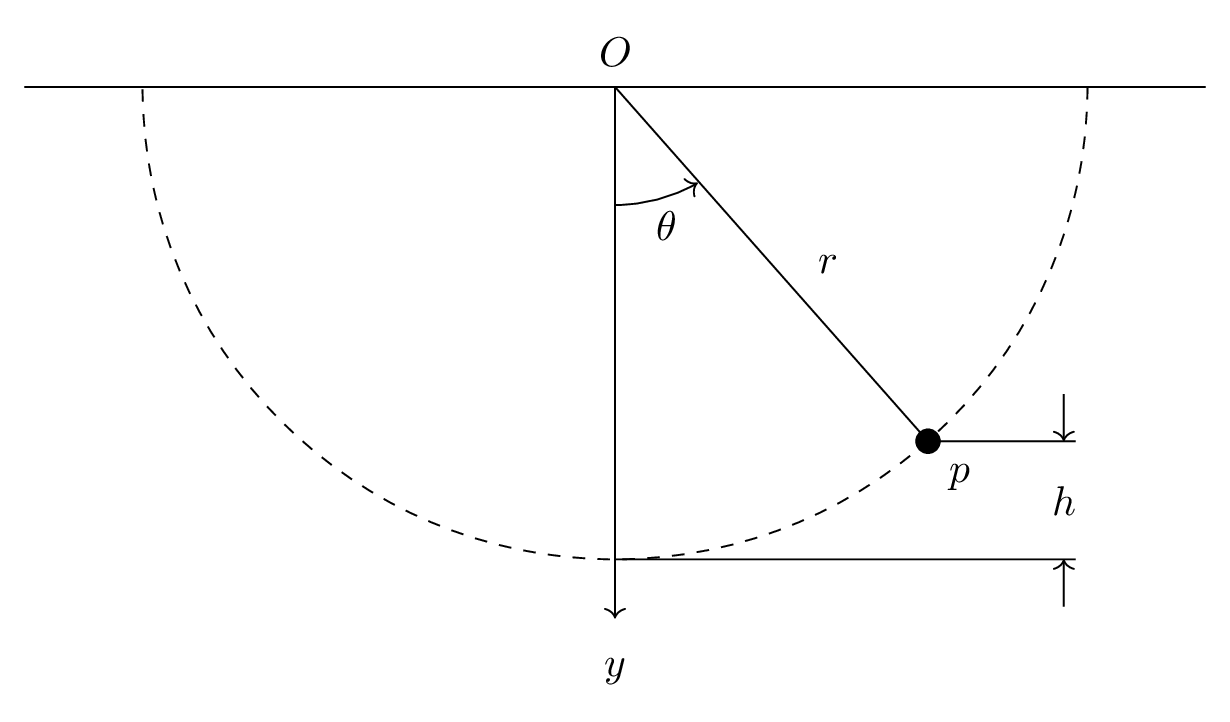
\includegraphics{Imagenes/pendulo_simple.pdf}
    \caption{Esquema del péndulo simple que oscila en un arco.}
    \label{fig:figura_pendulo_simple}
\end{figure}
\end{frame}
\begin{frame}
\frametitle{Organizando el problema}
Usando el eje coordenado, vemos que el ángulo polar $\theta$ varía de $-\pi/2$ a $\pi/2$, mientras que la coordenada radial $r = Op$ permanece constante.
\end{frame}
\begin{frame}
\frametitle{Organizando el problema}
Sea $g$ la aceleración debida a la gravedad y $W$ el peso del péndulo $p$.
\\
\bigskip
\pause
La energía potencial de $p$ en $\theta = 0$ es cero. Por lo que el valor de la energía potencial en cualquier instante, es el producto de $W$ por la altura $h$:
\begin{align*}
P = W (r - r \, \cos \theta)
\end{align*}
\end{frame}
\begin{frame}
\frametitle{Organizando el problema}
Mientras que la energía cinética viene dada por
\begin{align*}
K = \dfrac{m \, v^{2}}{2} = \dfrac{1}{2} \, \dfrac{W}{g} \left( r \, \dv{\theta}{t} \right)^{2}
\end{align*}
Como el péndulo está oscilando, la energía total es constante: $P + K = C$.
\end{frame}
\begin{frame}
\frametitle{Organizando el problema}
Lo que nos permite expresar una ecuación diferencial del movimiento:
\begin{align*}
W \, r (1 - \cos \theta) + \dfrac{1}{2} \dfrac{W}{g} \left( r \dv{\theta}{t} \right)^{2} = C
\end{align*}
\end{frame}
\begin{frame}
\frametitle{Condiciones para la ec. diferencial}
Para calcular $C$ tomamos el tiempo $t = 0$ cuando $\theta = \pi/2$, vemos que el péndulo está en reposo, por lo que $\dv*{\theta}{t} = 0$, cuando $t = 0$ y $\theta = \pi/2$.
\end{frame}
\begin{frame}
\frametitle{Ecuación de movimiento}
De esta manera $C = W \, r$ y la ecuación de movimiento resulta
\begin{align*}
\dfrac{r}{2 \, g} \left( \dv{\theta}{t} \right)^{2} - \cos \theta = 0
\end{align*}
\end{frame}
\begin{frame}
\frametitle{Consideración}
Como $p$ está oscilando de un lado a otro, $\dv*{\theta}{t}$ es en ocasiones positiva y en otras negativa; podemos estimar el período $T$, calculando el tiempo que tarda de ir de $\theta=0$ a $\theta=\pi/2$, para luego multiplicar el resultado por $4$.
\\
\bigskip
\pause
De esta manera podemos usar la raíz positiva para resolver la ecuación de $\dv*{\theta}{t}$.
\end{frame}
\begin{frame}
\frametitle{Resolviendo la ecuación diferencial}
Entonces tenemos
\begin{align*}
\sqrt{\dfrac{r}{2 \, g}} \, \dv{\theta}{t} &= \cos^{1/2} \theta \dd{t} = \\[1em]
\dd{t} &= \sqrt{\dfrac{r}{2 \, g}} \, \dv{\theta}{t} \cos^{-1/2} \theta \dd{\theta} = \\[1em]
T &= 4 \, \sqrt{\dfrac{r}{2 \, g}} \, \scaleint{6ex}_{\bs {0}}^{\pi/2} \cos^{-1/2} \theta \dd{\theta} = \\[1em]
\end{align*}
\end{frame}
\begin{frame}
\frametitle{Resolviendo la ecuación diferencial}
Entonces tenemos
\begin{align*}
&= 2 \, \sqrt{\dfrac{r}{2 \, g}} \, \scaleint{6ex}_{\bs {0}}^{\pi/2} 2 \, \sin^{0} \theta \, \cos^{-1/2} \theta \dd{\theta} = \\[0.8em]
&= \sqrt{\dfrac{2 \, r}{g}} \, B \left( \dfrac{1}{2}, \dfrac{1}{4} \right) = \\[0.8em]
&= \sqrt{\dfrac{2 \, r}{g}} \, \dfrac{\Gamma \left(\dfrac{1}{2} \right) \, \Gamma \left(\dfrac{1}{4} \right)}{\Gamma \left(\dfrac{3}{4} \right)} = 
\end{align*}
\end{frame}
\begin{frame}
\frametitle{Resolviendo la ecuación diferencial}
\begin{align*}
T = \sqrt{\dfrac{2 \, r}{g}} \, \dfrac{\Gamma \left(\dfrac{1}{2} \right) \, 4 \, \Gamma \left(\dfrac{5}{4} \right)}{\dfrac{4}{3} \, \Gamma \left(\dfrac{7}{4} \right)}
\end{align*}
Lo que nos falta es un paso: calcular los valores de la función Gamma.
\end{frame}
\end{document}